\begin{figure}[t]
    \centering
    % editable at https://docs.google.com/drawings/d/1nfqVV_dNqSV9g5UBuNopPLvubcEZx-vvg4K0ZCvNdfU/edit
    %\fig[.7]{CA-CAM}
    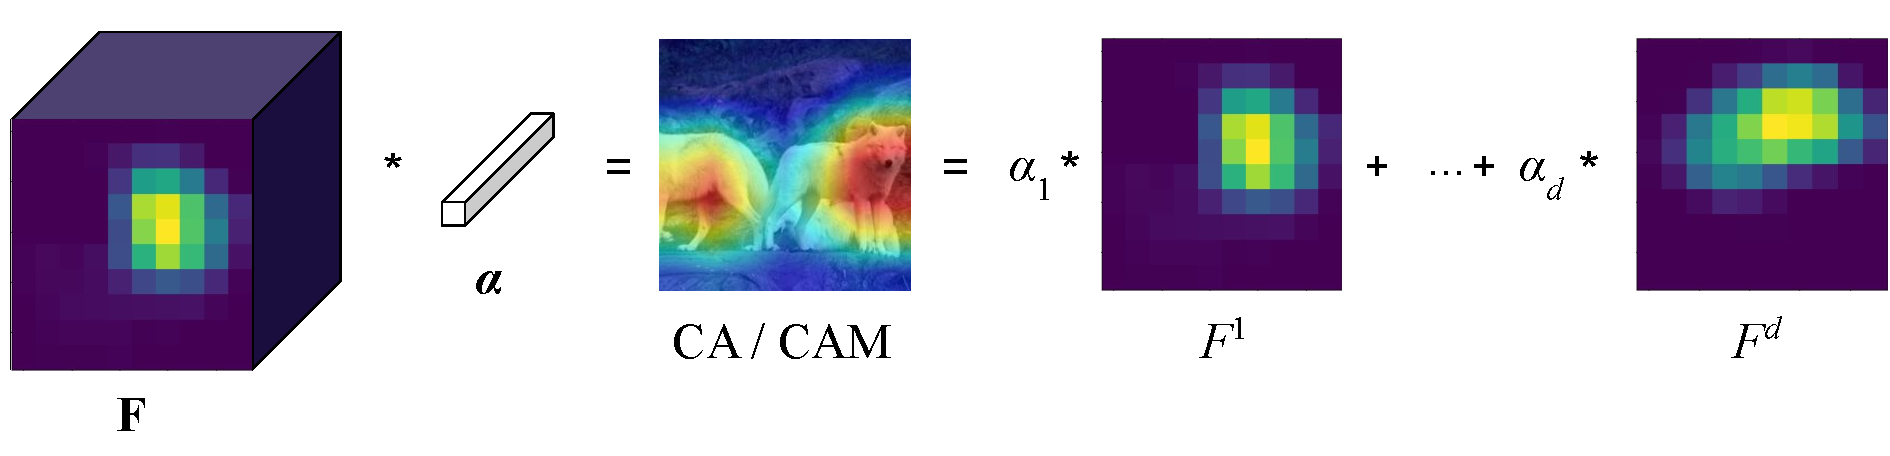
\includegraphics[width=.7\textwidth]{fig/castream/images/CA-CAM.pdf}
    \vspace{3pt}
    \caption{}
    %\emph{Visualization of eq.~\eq{connection}.} On the left, a feature tensor $\vF \in \real^{w \times h \times d}$ is multiplied by the vector $\valpha \in \real^d$ in the channel dimension, like in $1 \times 1$ convolution, where $w \times h$ is the spatial resolution and $d$ is the number of channels. This is \emph{cross attention} (CA)~\cite{dosovitskiy2020image} between the query $\valpha$ and the key $\vF$. On the right, a linear combination of feature maps $F^1, \dots, F^d \in \real^{w \times h}$ is taken with weights $\alpha_1, \dots, \alpha_d$. This is a \emph{class activation mapping} (CAM)~\cite{zhou2016learning} with class agnostic weights. Eq.~\eq{connection} expresses the fact that these two quantities are the same, provided that $\valpha = (\alpha_1, \dots, \alpha_d)$ and $\vF$ is reshaped as $F = (\vf^1 \dots \vf^d) \in \real^{p \times d}$, where $p = wh$ and $\vf^k = \vect(F^k) \in \real^{p}$ is the vectorized feature map of channel $k$.
    \label{fig:connection}
\end{figure}